% #############################################################################
% This is Chapter 6
% !TEX root = ../main.tex
% #############################################################################
% Change the Name of the Chapter i the following line
\fancychapter{System Evaluation}
\cleardoublepage
% The following line allows to ref this chapter
\label{chap:evaluation}

This chapter concerns the evaluation of the SmartFusion2 board and the developed prototype, its services, their performance, capabilities and limitations. The system and board were also evaluated regarding the fulfilled requirements, outlined in the previous chapter \ref{chap:problem}.

% -----------------------------------------------------
% -----------------------------------------------------
\section{Performance Tests}\label{chap:evaluation:performance}

The test objectives, configuration, results and conclusions are presented for every component tested.
The communication channel, device's security services and implemented services were tested.
Two performance metrics are used, the average test processing time, and the tested component's throughput.

% -----------------------------------------------------
\subsection{Testing configuration}\label{chap:evaluation:performance:config}

The tests were all performed on a Windows 10 computer, running the user software which calls the implemented PKCS\#11 API. The software communicates with the SmartFusion2 device through a UART serial port. The user software was used to run the tests.
Two applications were running on the computer while performing the tests, the PKCS\#11 application and the SoftConsole IDE, to run the code on the device.
For all tests, the serial port UART connection was configured with a 115200 bit/s baud rate, with 8 data bits, no parity bits and one stop bit.
Since the board does not provide a clock and API to measure elapsed time, the time had to be measured on the computer's side.
The elapsed time was measured using the function \texttt{gettimeofday()}, available in the C library \texttt{sys/time.h}.
Time measurement begins immediately before sending a message to the device, which triggers the service, and stops when the software receives a response, after it is finished.
In order to thoroughly study the performance and scalability of each component, the transmitted data size was varied, for components where it is logical and can potentially have a performance impact. The data size was tested, when possible, up to 36 KB, which is the maximum buffer size, limited by the 80 KB of RAM.
Obvious outlier values were excluded from the experimental calculations. The adopted rule was that values which are significantly above or below the average, and are never repeated were eliminated from the sample set.
Tests were performed in two different configurations.
For the first test configuration, the measured service is performed once in the device each transmission. This transmission is repeated multiple times, minimum thirty, for each set of values, until an acceptable variance is achieved. For most components the variance is well bellow 1\%.
For most components, the first configuration produced unstable results with a high variance, due to the communications overhead on every test run.
Thus, a second test configuration was applied on components, where the time to transmit messages needs to be minimized, to more accurately assess its isolated performance. For each transmission, the service was performed 100 consecutive times in the board. The resulting time was divided by 100 to obtain the average processing time.
With the second configuration, the results are visibly more stable.
An example of the difference between both configurations results, was on the AES tests. The first configuration's overhead, from the communications, compared to the second, resulted in higher time values of on average 15\%, with a peak 61\% overhead for the smallest data sizes.% Additionally when plotting the results, the second results scale almost perfectly linear, and the first results' are significantly more unstable.

% -----------------------------------------------------
\subsection{Performance models}\label{chap:evaluation:performance:models}

Some time results followed a close to perfect linear evolution, in function of the processed data size. In those cases, performance can be modeled with a formula composed of two different components \ref{eq:linear-eq}, a constant value independent of processed data, and a factor dependent on the processed data size.
\begin{equation}
	\label{eq:linear-eq}
	T_{Total} = T_{Constant} + T_{Data} * KB
\end{equation}
Linear regression was used to calculate both values, which are presented in tables when relevant. To assess the accuracy of the models, the median average percentage error was calculated and is presented next to its values. Tests which always process a fixed data size, such as, the ECC and KeyTree core services, only have a constant time component.

% -----------------------------------------------------
\subsection{Communications}\label{chap:evaluation:performance:comms}

In order to assess the communication channel performance, and its impact on the system, the average time to transmit data was measured. For each test, the computer application sent data of a specific size to the device, which returned an acknowledge message on reception. The test, in accordance with the first scenario, was repeated at least thirty times for each data size. The highest variance did not go above 0.2\%, for any value.
The average transmission times for each value are displayed in figure \ref{fig:comms:time}.
The values range from 0.048 seconds for 0.5 KB, to 3.2 s for 36 KB.
The performance, in milliseconds, can be modelled by a linear equation \ref{eq:linear-eq}, with values \(T_{total} = 7.281 + 88.638 * KB\), and a median average percentage error of 0.92 \%.

% \begin{figure}[h!]
%         \centering
%         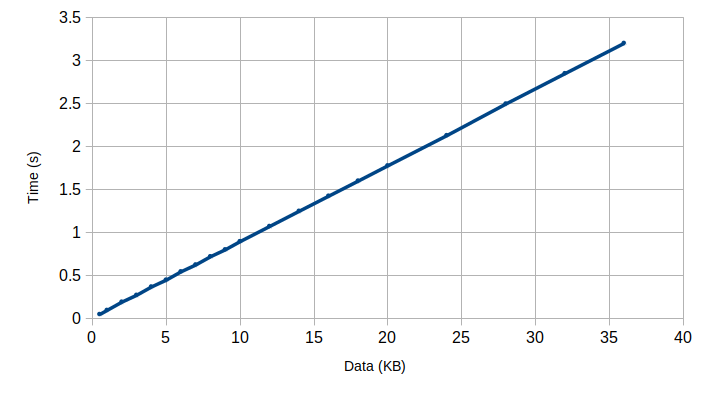
\includegraphics[width=0.7\textwidth]{./Images/comms-time.png}
%         \caption{Serial Port data transmission times}
%         \label{fig:comms:time}
% \end{figure}
%
% \begin{figure}[h!]
%         \centering
%         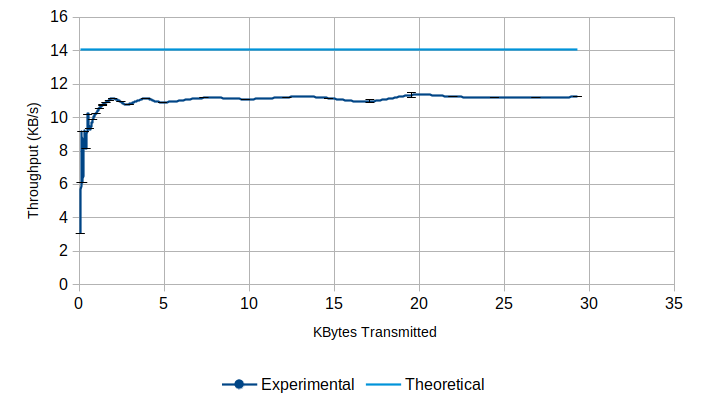
\includegraphics[width=0.7\textwidth]{./Images/comms-tput.png}
%         \caption{Serial port data transmission throughput}
%         \label{fig:comms:tput}
% \end{figure}
\begin{figure}[h!]
	\centering     %%% not \center
	\subfigure[Serial Port data transmission times]{\label{fig:comms:time}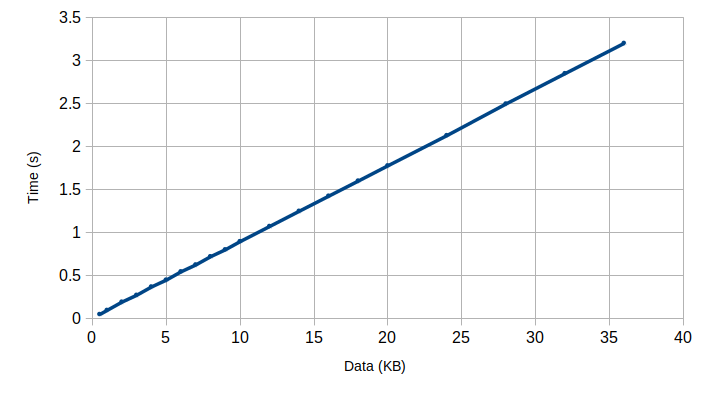
\includegraphics[width=79mm]{Images/comms-time.png}}
	\subfigure[Serial port data transmission throughput]{\label{fig:comms:tput}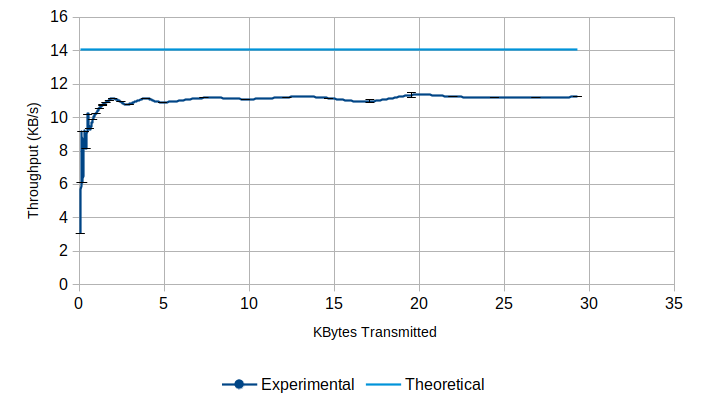
\includegraphics[width=79mm]{Images/comms-tput.png}}
	\caption{}
\end{figure}

For the subsequent graphic, the throughput was calculated from the transmission tests, for every test repetition.
Figure~\ref{fig:comms:tput} plots the experimental throughput and theoretical throughput. The theoretical throughput was calculated from the baud rate \(115200/8 = 14.06 KB/s\).
We can observe the experimental throughput starts at around 10 KB/s for smaller data sizes, and stabilizes around 11 KB/s, as size increases.
We can conclude the practical throughput is close to the theoretical, and as expected, stabilizes as the data size increases.

% -----------------------------------------------------
% -----------------------------------------------------
\subsection{SmartFusion2 Services}\label{chap:evaluation:board}

TODO - AES FPGA core test results!!!!

All the security accelerators of the SmartFusion2 SoC were tested. This includes the TRNG, AES, SHA, HMAC, KeyTree based SHA and ECC scalar multiplication and point addition services.
As discussed before, all services were tested using the two presented configurations. The services were tested taking into account three different time components \(T_{Total} = T_{Call} + T_{Transmittion} + T_{Service}\), with the first test configuration. The \(T_{Call}\) component is the elapsed for invoking the PKCS\#11 API, before any data is transmitted or the service is executed. From the results, we concluded this component's impact on performance is negligible, since it is practically always 0.
Predictably, the transmission time always follow the performance model studied in the previous section.
Thus, the following security core and implemented services tests focused on solely measuring the performance of the service on the device, without the data transmission part. To get a complete model of the overall systems' performance, from the user's perspective, the isolated service processing time can be added to the communications time.
Using the significantly more stable second test configuration, the isolated service processing time results are presented next.
Twenty different data sizes were used in the test, from 0.5 KB up to 36 KB.
All services followed a near perfect linear evolution, in function of the processed data size. Thus, linear regression was used to calculate the model values, presented in table \ref{tab:core-model}.

\begin{table}[h!]
\centering
\def\arraystretch{1.5}
\begin{tabular}{|c|c|c|c|c|c|c|c|}
\hline
Time (ms) & AES    & SHA    & HMAC   & TRNG   & KeyTree & ECC Add. & ECC Mult.	\\ \hline
Constant  & 0.489  & 0.498  & 0.783  & 0.368  & 1.655   & 7.204    & 545.381	\\ \hline
Data (KB) & 11.124 & 0.807  & 7.815  & 0.007  & -       & -	   & -		\\ \hline
MAE       & 0.12\% & 0.84\% & 0.13\% & 2.29\% & -       & -	   & -		\\ \hline
\end{tabular}
\caption{SmartFusion2 services time performance according to a linear model}
\label{tab:core-model}
\end{table}


All time values are presented in milliseconds, and the median average percentage error represents the error of the model's predicted values compared to the real results.
The AES service was tested with all possible variations. Namely, with 128 bit and 256 bit keys, with all four available modes and with encryption and decryption. Only one result is, shown since there was no variation among them. The AES mode, key size or encryption/decryption operation does not impact the performance. Therefore, there is no performance advantage in choosing CTR mode over CBC mode, or vice-versa.
Regarding the results, higher values of the time dependent factor, indicates the service time increases faster, as data sizes increase. Overall, the AES and HMAC total service time increases faster, compared to SHA, which increases significantly slower. The constant time is similar among the three services, HMAC is slightly higher.
The error percentages are all bellow 1\%, except for the TRNG service, proving the calculated models accurately represent all services' performance.
The TRNG service was tested by generating 16 random bytes, up to the maximum allowed by the API of 128 bytes. As expected the performance barely increases with the data size, and the constant factor is the most relevant for its performance.
The ECC services are the slowest performers, particularly the scalar multiplication (ECDH), with each run taking more than half a second.

\begin{figure}[h!]
	\centering
	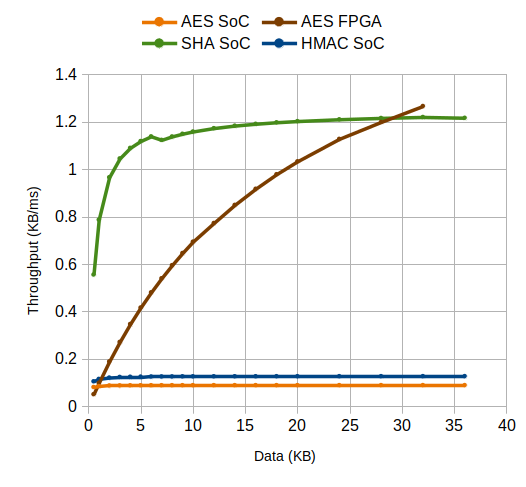
\includegraphics[width=0.7\textwidth]{./Images/core-tput.png}
	\caption{Security services throughput evolution}
	\label{fig:performance:core-tput}
\end{figure}

The graphic \ref{fig:performance:core-tput} represents the throughput calculated from the processing time results previously gathered. It shows all services throughput, shown in KB/ms, increases and eventually stabilizes at a specific value. AES stabilizes at around 1.2 KB/ms, and both SHA and HMAC at around 0.1 KB/ms.

% -----------------------------------------------------
% -----------------------------------------------------
\subsubsection{Core/Software Comparison}\label{chap:evaluation:services:software}

The SHA and HMAC performance difference results were enigmatic. The HMAC data dependent portion, 7.815 ms, is nearly 10 times higher than the SHA value, 0.807 ms. This means HMAC's time performance degrades nearly 10 times faster than the SHA performance. This is a surprising result, since the HMAC algorithm is composed of two hash computations and uses SHA-256, so the results are expected to be closer.
For this reason, a lightweight implementation of HMAC, SHA and AES was included in the board for comparison. The library used for HMAC and SHA was \cite{ogayHMAC}, and for AES \cite{tinycrypt}. 

\begin{figure}[h!]
	\centering
	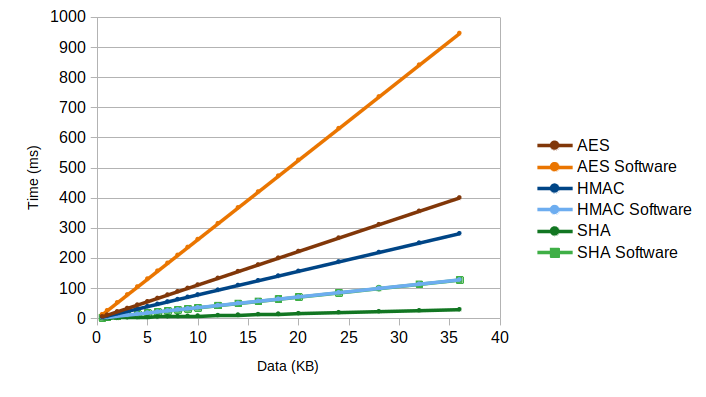
\includegraphics[width=0.7\textwidth]{./Images/software-core-time.png}
	\caption{Performance comparison of the board's cores and a software implementation}
	\label{fig:performance:software-core-time}
\end{figure}

The HMAC, SHA and AES software implementations were tested using the second test configuration.
Analyzing the time performance results in figure \ref{fig:performance:software-core-time}, the SHA and HMAC software results are almost identical, the HMAC is a slightly worse performer. Compared to the software results, the SHA core is significantly faster, and deteriorates very slowly as data size increases. The opposite happens for the HMAC core. It is convincingly a worst performer, compared to both HMAC and SHA software implementations. 
This is an ambiguous result, as there is no clear reason for the HMAC core performance degradation, compared to the SHA core and the software implementations. One could assume it could be caused by the DPA mitigations, but it would still not explain the meaningful discrepancy compared to the SHA core, which also includes these mitigations.
The AES software implementation was tested with encryption in CBC mode and a 256 bit key, as expected, it performs worse than the core service. CTR mode with the same configuration was also tested, and has very similar performance to CBC.

% -----------------------------------------------------
% -----------------------------------------------------
\subsubsection{Memory Performance}\label{chap:evaluation:services:memory}

The read and write performance of the different device's memories, along with the PUF service were tested. Both eSRAM and eNVM memories were tested from 0.5 KB to 36 KB. The PUF performance was tested from 16 bytes, up to its limit of 512 bytes. For the PUF and eNVM performance, due to the write cycle limitations, each test was performed with only 10 repetitions, compared to the usual 100 with the second configuration. Precautions were also taken, by changing the eNVM page being written for every repetition, to avoid exhausting any particular page.
The performance results in table \ref{tab:memory-model} were calculated according to a linear model.

\begin{table}[h!]
\centering
\def\arraystretch{1.5}
\begin{tabular}{|c|c|c|c|c|c|c|}
\hline
Time (ms) & RAM Op. & Write RAM & Read NVM & Write NVM & Fetch PUF & Enroll PUF \\ \hline
Constant  & 0.085     & 0.012     & 0.01     & 8.03      & 128.49    & 747.84  \\ \hline
Data (KB) & 0.34     & 0.014     & 0.02     & 298.10    & 0.006     & 0.008  \\ \hline
MAE       & 1.90\%    & 2.76\%    & 3.76\%   & 0.31\%    & 0.17\%    & 0.06\%  \\ \hline
\end{tabular}
\caption{Smartfusion2 memory performance time values according to a linear model}
\label{tab:core-model}
\end{table}


We can observe the PUF service barely fluctuates with the data size, since it is limited to 512 bytes per slot. The constant value is the significant portion, for both read and write performance.
The eNVM write performance deteriorates significantly with increasing data sizes, it is 298.10 ms slower per KB of data. The read performance is negligible.
The RAM write performance is comparable to the eNVM read performance. The RAM read performance was also tested, however, the results are not shown due to its extremely negligible and erratic performance. Instead, a simple increment operation test is presented, in order to show a benchmark for the RAM's performance.

% -----------------------------------------------------
% -----------------------------------------------------
\subsection{Implemented Services}\label{chap:evaluation:services}

All implemented services from chapter \ref{chap:implementation} were tested from data sizes of 0.5 KB up to 36 KB. Each service's performance depends on the used accelerator's, memory access and implemented logic.
The tested services were, encryption and authentication, decryption and authentication, both using the AES accelerator and the HMAC software implementation, the import keys service, using the AES, HMAC and PUF cores, ECDSA and ECDH, both using the ECC scalar multiplication accelerator. ECDSA also uses the ECC point addition core. It is worth noting, the encryption service also uses the TRNG service, to generate a random IV. The continuous encryption and decryption services, used AES in CBC mode, the HMAC software implementation and a 36 KB buffer for data. The services were tested with data sizes up to 200 KB.
Tests were performed with the second configuration, without data transmission, to test the processing time of the isolated services.
Similarly to the previous tests, the time performance results evolve linearly, so the equation components for each service were calculated using the linear regression algorithm. The obtained values are presented in table \ref{tab:services-model}.

\begin{table}[h!]
\centering
\def\arraystretch{1.5}
\begin{tabular}{|c|c|c|c|c|c|c|}
\hline
	Time (ms) & Encrypt Data  & Decrypt Data  & Import Keys & ECDSA & ECDH   \\ \hline
	constant  & 2.1    & 0.847  & 368.994  & 629.932 & 964.535 \\ \hline
	data      & 14.678 & 14.681 & 18.518 & 0.937 & - \\ \hline
	MAE	  & 0.10\% & 0.12\%  & 2.86\% & 0.18\% & - \\ \hline
\end{tabular}
\caption{Implemented services time values according to a linear model}
\label{tab:services-model}
\end{table}

% \begin{table}[]
% \centering
% \def\arraystretch{1.5}
% \begin{tabular}{|c|c|c|c|c|c|c|}
% \hline
% Time/Service   & Encrypt + MAC	  & Decrypt + MAC  & Import Keys & ECDSA   \\ \hline
%         constant (ms) & 29.413 & 29.413 & 0.002 & 0.138 \\ \hline
%         data (ms) & 6.704 & 6.704 & 1.942 & 1.542 \\ \hline
%         MAE \%	   & 1.032 & 1.006 & 0.127 & 1.760 \\ \hline
% \end{tabular}
% \caption{Implemented services throughput model values}
% \label{tab:services-model}
% \end{table}


Analyzing the results, both encryption/decryption and authentication services have very similar values, due to being based on the same service's and AES encryption and decryption having no discernible performance difference.
There is however a detectable difference in the constant component, due to the random IV generation with the board's TRNG on the encryption service.
The import keys service was tested up to 1 KB of key data, stored in RAM memory instead of eNVM. The generated MAC is stored in the PUF slot. The service was tested with 10 repetitions, instead of 100, to preserve eNVM write cycles.
The service performance barely varied, due to the small data interval. Its performance is pictured figure \ref{fig:performance:nvm-puf-time}, compared to the PUF and eNVM read and write performance. This figure is a good comparison for both key management options.
Key generation with ECDH and the SHA-based KeyTree derivation function performs at a constant 578.092 ms.
Scalar multiplication has a big impact on the performance for both ECDH and ECDSA.
The median average percentage error for the continuous encryption/decryption models is below 0.19\%, so the models almost perfectly represent its performance.% The import keys service model has the highest error with 2.86\%.
% The data dependent value, of both services, is extremely close to the sum of the previously calculated values of AES and HMAC, \(11.124+7.815=18.939\approx18.953\approx18.946\).
% The continuous operations are better performers due to using the faster HMAC software implementation, compared to the board's core.
% because of the HSM's 'RAM limitations, more demanding than other operations due to keys being storage in the same memory as the code. With 5 KB of key storage available, the system can store up to 20 symmetric keys of 32 bits, used to secure communications. However this can be bypassed by storing the keys in a high capacity external storage connected to the device. The keys are stored encrypted with internal keys, so they are secure.

\begin{figure}[h!]
	\centering
	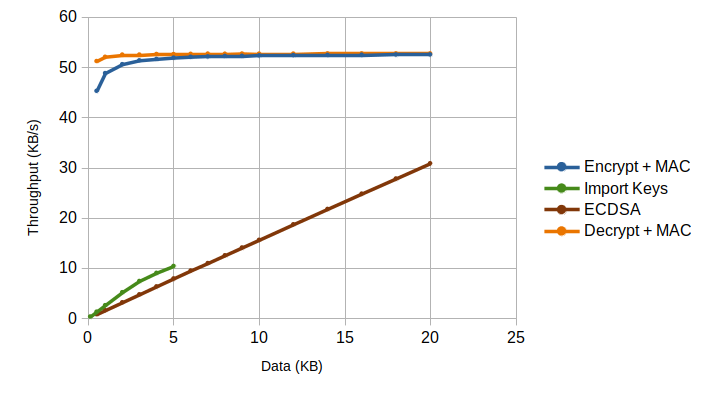
\includegraphics[width=0.7\textwidth]{./Images/services-tput.png}
	\caption{Continuous encryption and decryption throughput evolution for increasing input data sizes}
	\label{fig:performance:services-tput}
\end{figure}

Figure \ref{fig:performance:services-tput} plots the throughput (KB/s) values for the continuous encryption and decryption services. Throughput steadily increases and stabilizes after 10 KB, at around 68 KB/s, for both services.
The continuous encryption/decryption implementation raises an efficiency question. An optimal buffer size must be chosen. The previous tests were performed with a 36 KB buffer.
To answer this, the impact of the buffer size on performance must be studied.
This was achieved by performing the same test on the continuous encryption service, with varying buffer sizes, from 0.1 KB up to 35 KB. Picture \ref{fig:performance:buffer-tput} shows the maximum, average and minimum throughput for each buffer size.
All tests revealed the same linear performance behaviour as the previous test with a 36 KB buffer. The worst performance, and therefore lower throughput, is achieved with low data sizes of 0.5 KB. The time evolution is linear, and the throughput eventually stabilizes around its maximum value, with data sizes higher than 20 KB.
A smaller range from the minimum to maximum throughput, for a particular buffer size, indicates the throughput increases slower, as data size increases.

\begin{figure}[h!]
	\centering
	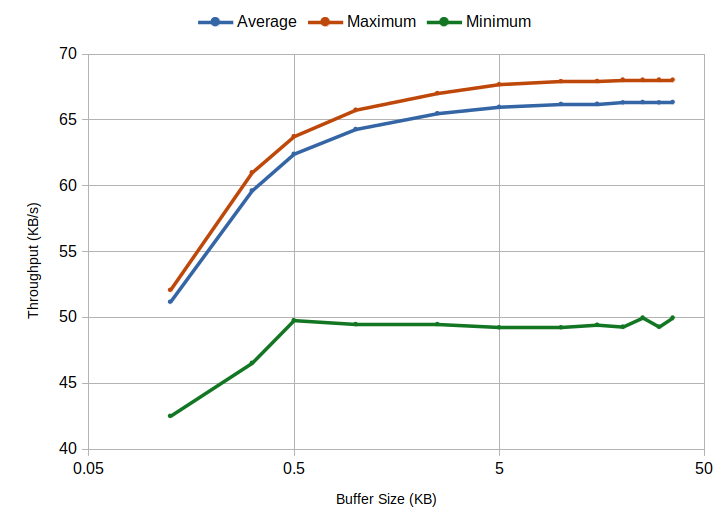
\includegraphics[width=0.7\textwidth]{./Images/buffer-tput.png}
	\caption{Continuous encryption throughput evolution with increasing buffer sizes}
	\label{fig:performance:buffer-tput}
\end{figure}

% \begin{figure}[h!]
%         \centering     %%% not \center
%         \subfigure[Constant component overhead \% of total performance]{\label{fig:performance:buffer-overhead}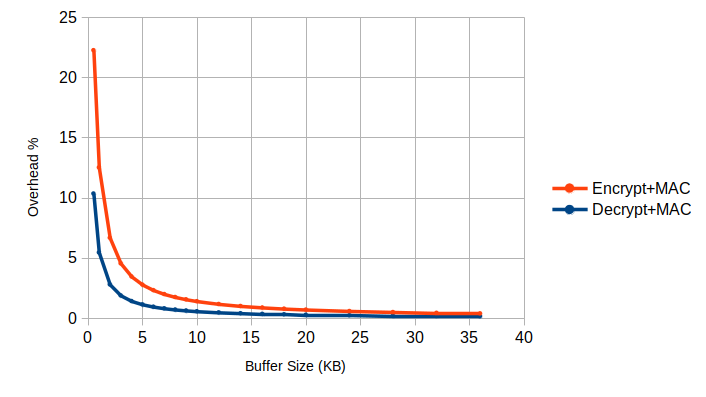
\includegraphics[width=79mm]{./Images/buffer-overhead.png}}
%         \subfigure[Throughput evolution from buffer size]{\label{fig:performance:buffer-tput}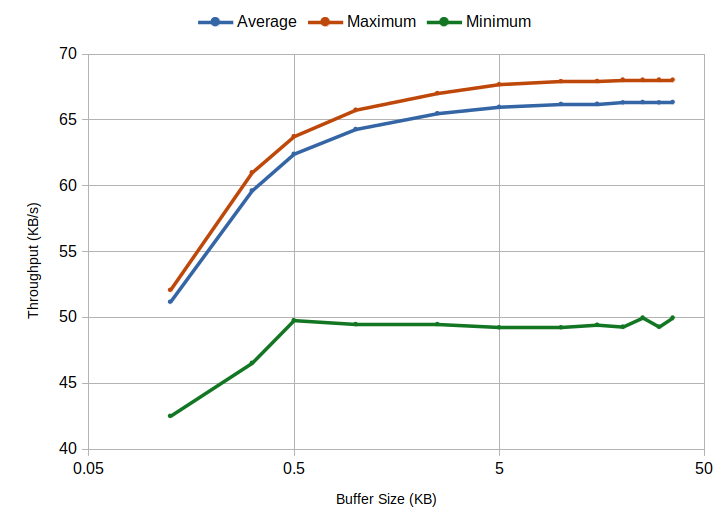
\includegraphics[width=79mm]{./Images/buffer-tput.png}}
%         \caption{Buffer size overhead and throughput evolution}
% \end{figure}

Analysing the plot, the average throughput significantly increases from 0,1 KB up until 5 KB, after which, the average throughput stabilizes around 66 KB/s and the maximum at 68 KB/s. The minimum throughput stabilizes around 49.5 KB/s, after a buffer size of 0.5 KB. If the goal is to maximize throughput, there is no advantage in using a buffer bigger than 10 KB. Even a 5 KB buffer has almost identical performance. Additional trade-offs can be implemented, if the total data size the system will process is known beforehand. For higher data sizes, where the maximum throughput is achieved, the optimal buffer size is 10 KB. However, if the system mainly receives small data of around 0.5 KB, the minimum throughput becomes relevant. It becomes stable from a buffer of 0.5 KB, up to a 35 KB. For this use case, if memory space is needed, a 0.5 KB buffer is acceptable. The extra saved memory can be used to implement more functionalities.


% TODO
% The results in table~ for the encryption and decryption operations are very similar due to both using the same board services, AES encryption and HMAC, but in a different order. It is also important to note AES encryption and decryption in CTR mode is essentially the same operation due the mode's characteristics.
% Relating to the variation in data size, the values vary between approximately 0.1284 and 0.1825 seconds, which is a very insignificant difference. Thus we can conclude, the data size has a negligible impact on the operations performance.

% Regarding the key generation operation results in table~, two values were obtained through different methods. Due to the operation using SRAM-PUF services to enroll new keys in the eNVM memory, with limited write cycles and key slots, this operation cannot be repeated enough times to get a relevant enough sample size.
% So a trade off was achieved. The operation was performed 1000 times without the key enrollment operation, meaning only the ecdh key generation algorithm and key derivation function (SHA-256).
% Since the enrollment phase is presumed to be expensive, due to writing in eNVM memory, the test was also performed 10 times with key enrollment, to get an idea of its potential performance cost.
% This result is congruent with the one obtained by \cite{parrinha2017flexible} of 0.57s per ECC scalar multiplication.

% -----------------------------------------------------
% -----------------------------------------------------
\section{Requirements}\label{chap:evaluation:requirements}

This section evaluates the fulfilled requirements of the developed system, defined in chapter \ref{chap:problem:requirements}.
Firstly, the chosen device SmartFusion2 SoC is a portable board, with a robust set of security services.
Compared to the existing HSMs on the market, this device is one of the cheapest, so it is adequate for distribution among several users. Market HSMs go from 650€ up to \$39,000 \cite{HSMpriceArticles}, \cite{HSMPresentationPrices}. A M2S090TS SmartFusion2 evaluation kit is priced at 384 € \cite{smartfusionPrice}.
Regarding its services, it provides encryption and authentication with AES and HMAC, a secure storage service for keys, SRAM-PUF, and ECC primitives for shared keys with ECDH and digital signatures, by implementing ECDSA. It provides tamper detection capabilities and data zeroization.
It has the necessary functionalities to provide authentication and confidentiality to communications, which is the main requirement of the system.
The prototype uses the board's services, except for the HMAC software implementation, and all keys are stored securely.
The developed key management solution allows the periodic replacement of keys. Therefore, communications with new entities, with similar devices, can be established.
Users must authenticate themselves to the device, using its authentication PIN. This way entities can manage which users have access to the device, in behalf of the entity.
Whenever a tamper attempt or error is detected, the device is blocked and does not allow commands, and eventually is completely erased, if deemed necessary. Any potential attacks and data leaks data are prevented.
A PKCS\#11 API was developed to expose the device's features and increase device interoperability. For users, an easy-to-use command line interface application, which calls the implemented PKCS\#11 API, was implemented.

% -----------------------------------------------------
% -----------------------------------------------------
\section*{Summary}\label{chap:evaluation:summary}

In this chapter, the implemented system performance was thoroughly tested. Starting with the communication channel performance, following will all the SmartFusion2 security cores and implemented services. All the performance tests were isolated from the communications channel performance. Performance models which accurately represent each service performance, were calculated and presented. All the models allows anyone using these device, to accurately study and predict the performance of a custom service, implemented on the board. Therefore, this chapter provides a robust study of the SmartFusion2 board, its services characteristics, performance, as well as possible services to implement, feature trade offs and efficiency concerns.
